\documentclass{article}

\usepackage{amsmath} % math stuff
\usepackage{amssymb} % math stuff
\usepackage{array} % equations and stuff
\usepackage{bm} % bold math
%\usepackage{caption} % suppressed table numbering; incompatible with revtex, and longtable, I think
\usepackage{comment} % comment environment
%\usepackage{enumitem} % customization of enumeration, itemize, and description
\usepackage[T1]{fontenc} % font encoding for special characters, must also use scalable font package
\usepackage[margin=0.8in]{geometry} % paper sizes and margins (but be careful not to mess up pre-defined pages)
\usepackage{graphicx} % for graphics
%\usepackage{helvet} % default font is the helvetica postscript font
\usepackage{layouts} % print units like widths
\usepackage{lipsum} % lorem ipsum filler text
\usepackage{lmodern} % scalable font?
\usepackage{longtable} % multi-page tables
\usepackage{mathrsfs} % math script font
\usepackage{mhchem} % easier chemical formula
\usepackage{microtype} % allows disabling of ligatures
%\usepackage{newcent} % new century schoolbook font
\usepackage{nicefrac}
\usepackage{parskip} % removes paragraph indentation, and adjusts paragraph skip, as well as list items
%\usepackage{setspace} % adjust text spacing and indents
\usepackage{siunitx} % decimal alignment
\usepackage{subfigure} % divided figures
%\usepackage{tabu} % extra table options
\usepackage{textcomp} % symbols
\usepackage{threeparttablex} % better footnotes with longtable
\usepackage{titling} % title placement
\usepackage{ulem} % strikethrough text
%\usepackage{url} % superceded by hyperref
\usepackage{verbatim} % verbatim environment
\usepackage{xcolor} % colors and color boxes
\usepackage{xspace} % commands that don't eat up white space
\usepackage{hyperref} % links and page setup; should always come last

\hypersetup{
	bookmarks=true,
	colorlinks=true,
	citecolor=blue,
	linkcolor=blue,
	urlcolor=blue,
	pdfstartview={XYZ null null 1.0} % default open view is 100%
}

\DisableLigatures[f]{encoding = *, family = * } % disable ff, fi, fl ligatures, without f option, it also disables -- = endash
\renewcommand{\arraystretch}{1.1} % extra vertical space in tables

\begin{document}

\pagestyle{empty} % don't number pages

% custom title
\begin{center}
{\LARGE Classic Riddler}

\vspace{0.15in}

{\Large 9 October 2020}
\end{center}


\section*{Riddle:}

Parking cars is one thing---parking trucks is another thing entirely.
Suppose I'm driving a \textit{very long} truck (with length $L$) with two front wheels and two rear wheels.
(The truck is so long compared to its width that I can consider the two front wheels as being a single wheel, and the two rear wheels as being a single wheel.)

Question 1: Suppose I can rotate the front wheels up to 30 degrees in either direction (right or left), but the rear wheels do not turn.
What is the truck's turning radius?

Question 2: Suppose I can also rotate the rear wheels---independently from the front wheels---30 degrees in either direction.
\textit{Now} what is the truck's turning radius?

\section*{Solution:}

This is a basic geometry problem.
In principle, for an infinitely thin vehicle with just two infinitely thin wheels (one each at the front and back), the wheels move exactly along their orientation.
With this motion, the centers of the wheels (i.e., where the wheels touch the ground) trace out concentric circles.
The center of the circles is where lines normal to the wheels meet, and these lines are the radii of the circles.
For a real car, this is only approximate; while each wheel moves in a circle, its orientation is not exactly normal to the radius (and thus the motion of the each wheel is not strictly along its own orientation).

For the specific cases in this riddle, I have created the two diagrams below.
The truck (of length $L$ is in blue, and the turned wheels are in red.
The two normal lines originating from the wheels come to a point at $c$, the mutual center of the circles the wheels trace out, and these lines along with the truck form a triangle.
Using basic geometry, it is possible to identify the lengths of all the sides of the triangle.

\vspace{0.2in}
\begin{center}
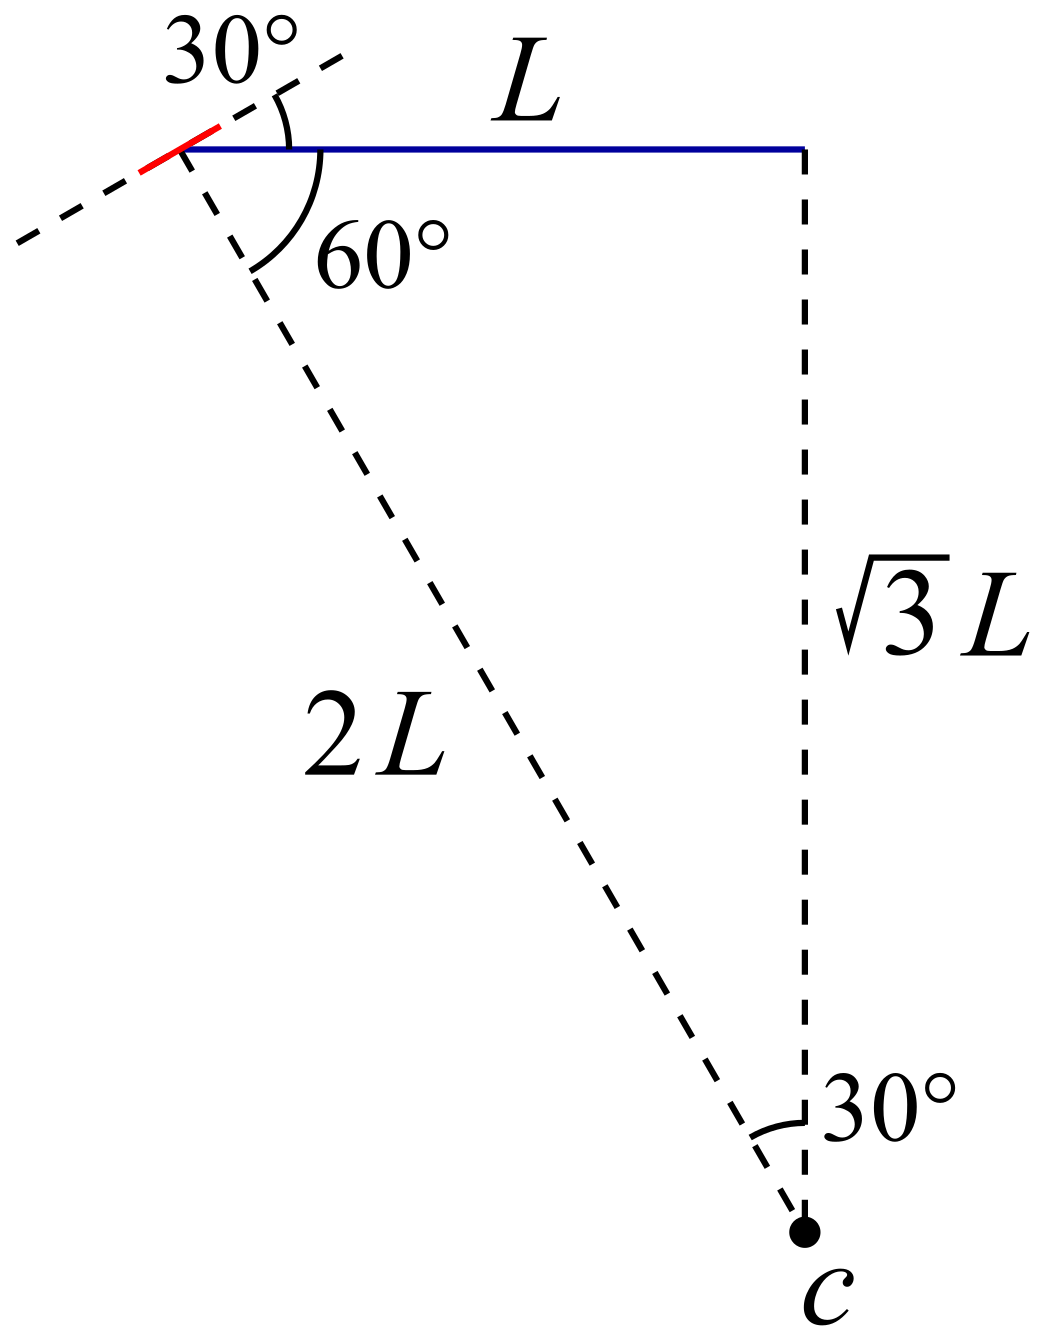
\includegraphics[height=2.8in]{turning_1.png}
\hspace{0.6in}
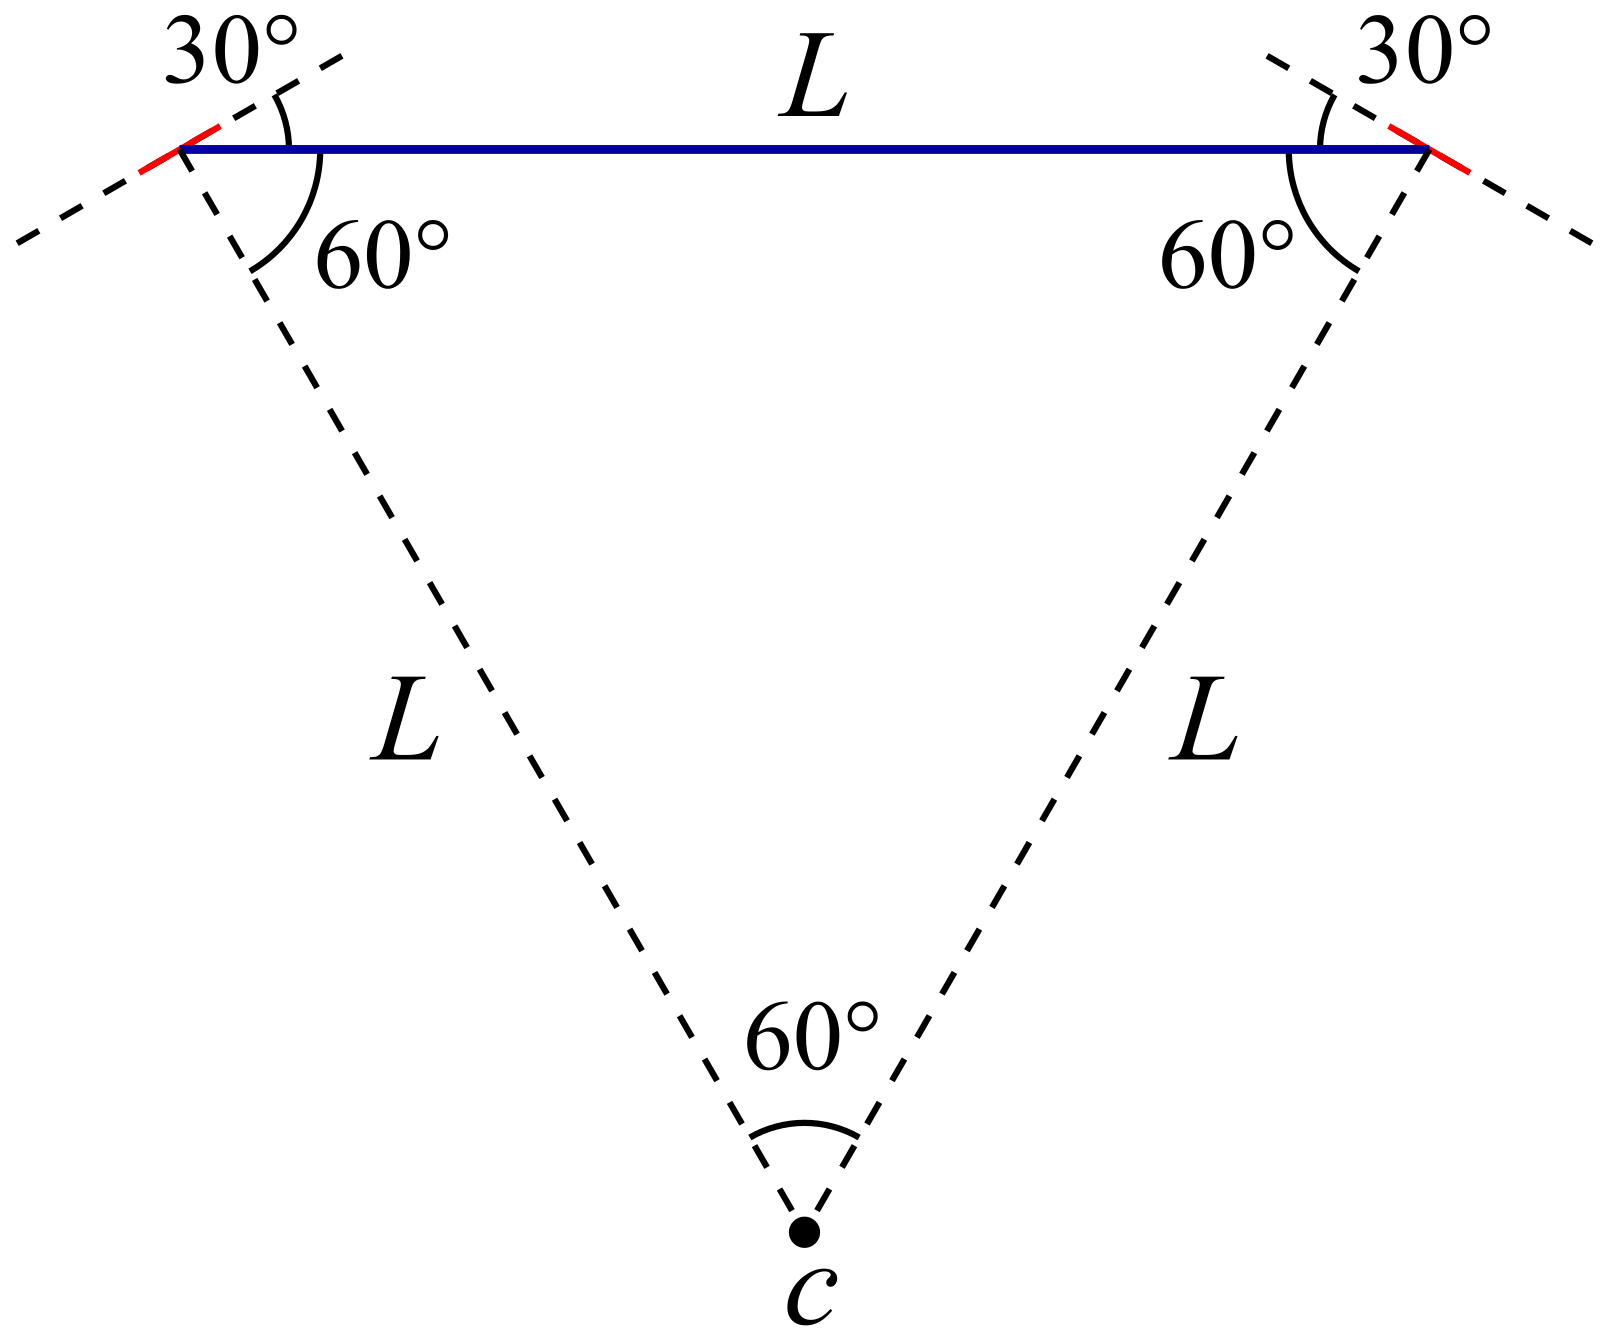
\includegraphics[height=2.8in]{turning_2.png}
\end{center}
\vspace{0.2in}

According to the link from the riddle, the turning radius is defined as the outermost radius that a vehicle uses to make a full turn.
Thus, the solution to the riddle is the length of the longest triangle side.
So the solutions are
\fcolorbox{red}{white}{$\bm{2L}$} for the first question and
\fcolorbox{red}{white}{$\bm L$} for the second question.


\end{document}